\begin{enumerate}[label=\thesubsection.\arabic*.,ref=\thesubsection.\theenumi]
\numberwithin{equation}{enumi}
\item
For the Wein-bridge oscillator of Fig \ref{fig:ee18btech11044_3_tikz_1}, use the expression for loop gain in Eq \ref{eq:ee18btech11044_3_1}  to find the poles of the closed-loop system. Give the expression for the pole , Q and use it to show that to locate the poles in the right half of s plane, $\frac{R_2}{R_1}$ must be selected to be greater than 2. 

\begin{figure}[!hbt]
	\begin{center}
			\resizebox{\columnwidth}{!}{\begin{circuitikz}
\ctikzset{bipoles/length=1cm}

\draw 
(0, 0) node[op amp] (opamp) {}
(opamp.-) -- (-1,0.35) -- (-1.5,0.35) to[R=$R_1$] (-3,0.35) -- (-3,0.33)node[ground]{}
(-1,0.35)-- (-1,1) to[R=$R_2$] (2,1) -- (2,0){}
(opamp.out)--(2,0){}
(opamp.+) -- (-1,-0.35) -- (-1,-1.5) to[C=$C$] (0.5,-1.5) to[R=$R$] (2,-1.5) -- (2,0){}
(-1,-1.5) -- (-1,-1.75)to[R=$R$] (-1,-2.5) -- (-1,-2.57)node[ground]{}
(0.5,-1.5) -- (0.5,-1.75) to[C=$C$] (0.5,-2.5) -- (0.5,-2.57)node[ground]{}
node at (2.3,0){$V_{out}$}



;\end{circuitikz}
}
	\end{center}
\caption{}
\label{fig:ee18btech11044_3_tikz_1}
\end{figure}


\item Compare the basic structure for a sinusoidal oscillator with Wein-bridge oscillator and give expressions for G and H. 

\solution
\begin{itemize}
    \item Comparring Fig \ref{fig:ee18btech11044_3_tikz_1} and Fig \ref{fig:ee18btech11044_3_tikz_2}, we get
\begin{align}
G = 1+\frac{R_2}{R_1} \\
H = \frac{Z_p}{Z_p + Z_s}
\end{align}
where,
\begin{align}
    Z_p = \frac{R}{RSC+1} \\
    Z_s = \frac{RSC+1}{SC}
\end{align}
\end{itemize}



\begin{figure}[!hbt]
	\begin{center}
		\resizebox{\columnwidth}{!}{\tikzstyle{block} = [draw, fill=white!20, rectangle, 
    minimum height=3em, minimum width=6em]
\tikzstyle{sum} = [draw, fill=white!20, circle, node distance=1cm]
\tikzstyle{input} = [coordinate]
\tikzstyle{output} = [coordinate]
\tikzstyle{pinstyle} = [pin edge={to-,thin,black}]

\begin{tikzpicture}[auto, node distance=2cm,>=latex']
    \node [input, name=input] {};
    \node [sum, right of=input] (sum) {};
    \node [block, right of=sum] (controller) {$G(s) = 1 + \frac{R_2}{R_1}$};
    \node [output, right of=controller] (output) {};
    \node [block, below of=controller] (feedback) {$H(s) = \frac{Z_p}{Z_p+Z_s}$};
    
    \draw [->] (sum) -- node {$V_i$} (controller);
    \draw [->] (controller) -- node [name=y] {$V_o$}(output);
    \draw [->] (y) |- (feedback);
    \draw [->] (feedback) -| node[pos=0.99]{$+$}  node [near end] {$V_f$} (sum);
\end{tikzpicture}
}
	\end{center}
\caption{}
\label{fig:ee18btech11044_3_tikz_2}
\end{figure} 





\item
Give the expression for loop gain for Wein-bridge oscillator. 

\solution
\begin{align}
    T(s) = A(s) \beta(s) \\ 
    T(s) = \frac{1+\frac{R_2}{R_1}}{1 + Z_s Y_p} \\
    T(s) = \frac{1+\frac{R_2}{R_1}}{1 + (\frac{sRC + 1}{sC}) (\frac{sRC+1}{R})} \\
    T(s) = \frac{1+\frac{R_2}{R_1}}{1 + \frac{s^2R^2C^2 +sRC + sRC + 1}{sRC}} \\
    T(s) = \frac{1 + \frac{R_2}{R_1}}{3 + sCR + \frac{1}{sCR}} \label{eq:ee18btech11044_3_1}
\end{align}

\item Write the characteristic equation for Wein-bridge oscillator.

\solution
\begin{align}
    1 - T(s) = 0  \\
    1 - \frac{1 + \frac{R_2}{R_1}}{3 + sCR + \frac{1}{sCR}} = 0  \\
    3 + sRC + \frac{1}{sCR} = 1 + \frac{R_2}{R_1}  \\
    3 - 1 +sRC +\frac{1}{sRC} -\frac{R_2}{R_1} = 0  \\
    2s + s^2 RC + \frac{1}{RC} -s\frac{R_2}{R_1} = 0  \\
    s^2 RC + s(2 - \frac{R_2}{R_1}) + \frac{1}{RC} =0 \\
    s^2 + s \frac{1}{RC}(2-\frac{R_2}{R_1}) + \frac{1}{R^2C^2} = 0 \label{eq:ee18btech11044_3_2}
\end{align}

\item
Write the general expression for the characteristic equation.

\solution
\begin{align}
    s^2 + s\frac{\omega_0}{Q} + \omega_0^2 = 0 \label{eq:ee18btech11044_3_3}
\end{align}

\item State the \textbf{Barkhausen criterion} for sustained oscillations with frequency $\omega_0$.

\solution
\begin{align}
    T(j\omega_0) = G(j\omega_0)  H(j\omega_0) = 1
\end{align}
\begin{itemize}
    \item That is, at $\omega_0$ the phase of the loop gain should be zero and the magnitude of loop gain should be 1.
    \item Only for a $\infty$ gain,system will produce a finite output for zero input. 
\end{itemize}

\item Give the definition of \textbf{Quality factor}(Q) and explain its significance.

\solution
\begin{itemize}
    \item It is a parameter of an oscillatory system expressing the relationship between stored energy and energy dissipation.
    \item The "purity" of output sine waves will be a function of the selectivity feedback network.
    \item That is, higher the value of Q for frequency selective network, the less the harmonic content of sine wave produced.
\end{itemize}
 


\item 
Compare the equations \ref{eq:ee18btech11044_3_2} and \ref{eq:ee18btech11044_3_3} and give expressions for Q and $\omega_0$

\solution
\begin{align}
    \omega_0^2 = \frac{1}{R^2C^2} \\
    \omega_0 = \frac{1}{RC} \label{eq:ee18btech11044_3_4} \\
    \frac{\omega_0}{Q} = \frac{1}{RC}(2 - \frac{R_2}{R_1}) \\
    Q = \frac{1}{(2 - \frac{R_2}{R_1})} \label{eq:ee18btech11044_3_5} \\
\end{align}
\item 
Using Eq \ref{eq:ee18btech11044_3_5} calculate the value of $\frac{R_2}{R_1}$ for which poles lie on right hand of s-plane.

\solution 

Poles lie on imaginary axis for $Q = \infty$
\begin{align}
    2 - \frac{R_2}{R_1} = 0 \\
    \frac{R_2}{R_1} = 2
\end{align}
$\therefore$ For poles to lie on right hand side of s-plane
\begin{align}
    \frac{R_2}{R_1} >2
\end{align}


\item
Verify the above calculations using a Python code.

\solution
\begin{lstlisting}
codes/ee18btech11044_3_1.py
\end{lstlisting}
\begin{itemize}
    \item This figure shows how the location of poles vary if $\frac{R_2}{R_1}$ is varied for a fixed $\omega_0$.
    \item I have varied $\frac{R_2}{R_1}$ from -10 to 10. 
\end{itemize}

\begin{figure}[!ht]
\centering
\includegraphics[width=\columnwidth]{./figs/ee18btech11044/ee18btech11044_3_1.eps}
\caption{}
\end{figure}


\item Simulate the circuit shown in Fig \ref{fig:ee18btech11044_3_tikz_1} using spice simulators. Plot the output generated using python.

\solution

You can find the netlist for the simulated circuit here:

\begin{lstlisting}
spice/ee18btech11044.net
\end{lstlisting}

You can find the python script used to generate the output here:

\begin{lstlisting}
codes/ee18btech11044_spice.py
\end{lstlisting}

\begin{figure}[!ht]
\centering
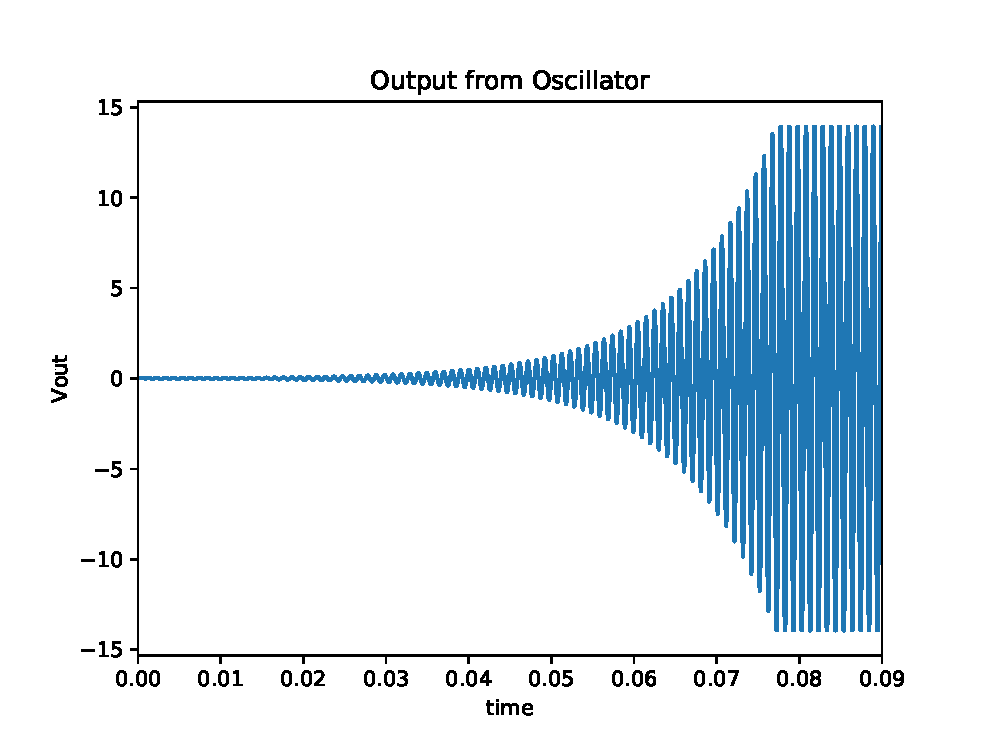
\includegraphics[width=\columnwidth]{./figs/ee18btech11044/ee18btech11044_3_2.eps}
\caption{}
\end{figure}

\item Tabulate the values of Resistors and Capacitors you have chosen for the simulation.

\solution

\begin{table}[!ht]
\centering
\input{./tables/ee18btech11044/ee18btech11044_3_t_1.tex}
\caption{}
\label{table:ee18btech11044_t_1}
\end{table}

Where, according to Fig \ref{fig:ee18btech11044_3_tikz_1}
\begin{align}
    R_p = R_s = R \\
    C_p = C_s = C
\end{align}
 
 \item Calculate the frequency of sinusoidal generated for the combination of R and C chosen using Eq \ref{eq:ee18btech11044_3_4}
 
 \solution
 
 Frequency generated is given by 
 
 \begin{align}
     \omega_{0} = \frac{1}{ R C} \\
     \omega_{0} = 6250 rad/sec \\
     f_{0} = 995.22Hz.
 \end{align}
 
 \item Calculate the frequency of sinusoidal wave using plot generated from simulation.
 
 \solution
 \begin{itemize}
     \item Consider a part of plot generated from simulation shown in the Fig \ref{fig:ee18btech11044_3_plot_3}.
     \item Calculating the Time-period of the sinusoidal wave generated using the two points marked in the Fig \ref{fig:ee18btech11044_3_plot_3}.
     \begin{align}
         T_0 = 0.0856452 - 0.0846361 \\
         f_0 = 1/T_0 \\
         f_0 = 990.98Hz.
     \end{align}
     \item We get the frequencies calculated from the formulae and the plot to be approximately same.
 \end{itemize}
 
 
 \begin{figure}[!ht]
\centering
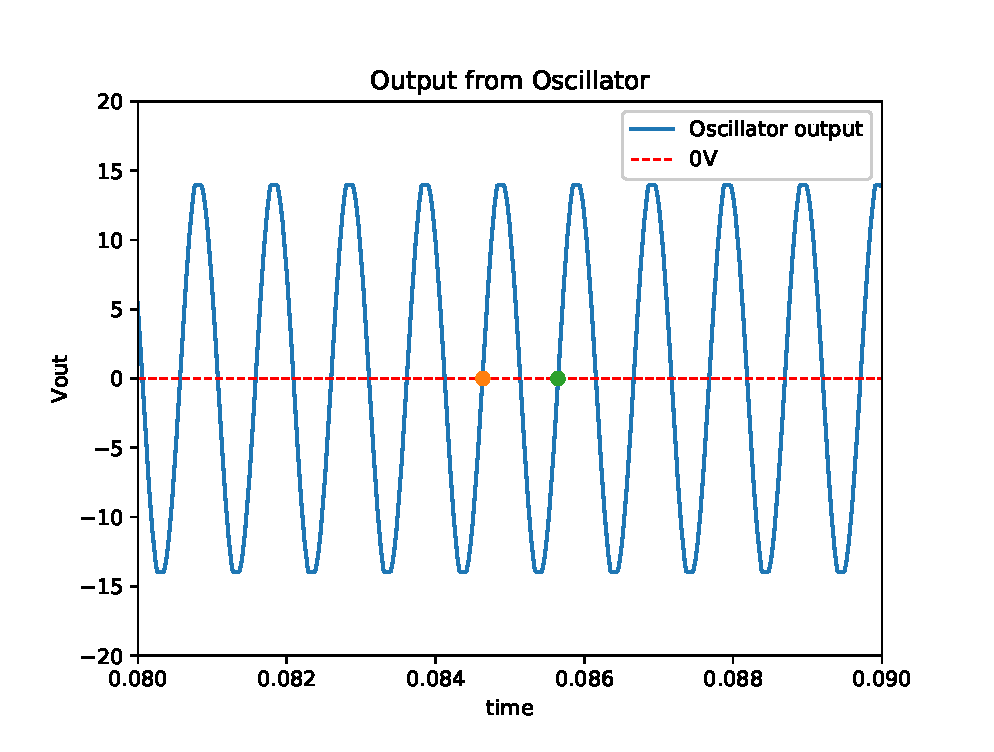
\includegraphics[width=\columnwidth]{./figs/ee18btech11044/ee18btech11044_3_3.eps}
\caption{}
\label{fig:ee18btech11044_3_plot_3}
\end{figure}
\end{enumerate}
